\exercise

Let us given the integer array $A = [ 3, 8, 2, 1, 9, 5, 11, 15 ]$
%
\begin{enumerate}

  \item Show how to turn the Range Minimum Query (RMQ) problem over the generic
  integer array $A$ into a RMQ problem over an array $B$ formed by entries
  $\pm 1$.

  \item  Build a data structure that solves the RMQ problem over $B[1, n]$ using
  space $O(n \log n)$ and $O(1)$ query time.

  \item Show how to solve $\text{RMQ}_A(5, 7)$ over the data structure built on
  $B$.

\end{enumerate}

\solution

\begin{enumerate}

  \item We have to reduce the RMQ problem into an LCA one. To obtain this, we
  first construct the \emph{cartesian tree} of $A$, $\mathcal{C}_A$, which is
  shown in \autoref{fig:cartesian-tree}.
  %
  \begin{figure}[b]
    \centering
    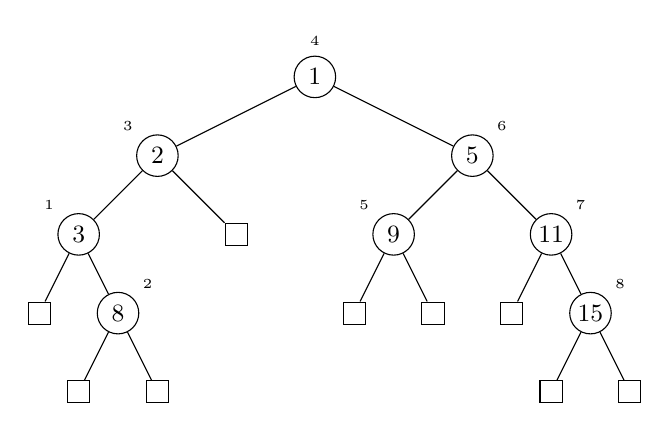
\begin{tikzpicture}[
      grow=down,
      inner/.style={thin, draw, inner sep=0, minimum size=15, circle},
      leaf/.style={thin, draw, fill=white, inner sep=0, minimum size=8},
      phantom/.style={draw=none, fill=none},
      level 1/.style={sibling distance = 4cm, level distance = 1cm},
      level 2/.style={sibling distance = 2cm, level distance = 1cm},
      level 3/.style={sibling distance = 1cm, level distance = 1cm},
      every edge/.style={-, thin}
    ]
    \node[inner, label=above:{\tiny 4}] {\small 1}
    child {
      node[inner, label=above left:{\tiny 3}] {\small 2}
      child {
        node[inner, label=above left:{\tiny 1}] {\small 3}
        child {
          node[leaf] {}
          edge from parent[-]
        }
        child {
          node[inner, label=above right:{\tiny 2}] {\small 8}
          child {
            node[leaf] {}
            edge from parent[-]
          }
          child {
            node[leaf] {}
            edge from parent[-]
          }
          edge from parent[-]
        }
        edge from parent[-]
      }
      child {
        node[leaf] {}
        edge from parent[-]
      }
      edge from parent[-]
    }
    child {
      node[inner, label=above right:{\tiny 6}] {\small 5}
      child {
        node[inner, label=above left:{\tiny 5}] {\small 9}
        child {
          node[leaf] {}
          edge from parent[-]
        }
        child {
          node[leaf] {}
          edge from parent[-]
        }
        edge from parent[-]
      }
      child {
        node[inner, label=above right:{\tiny 7}] {\small 11}
        child {
          node[leaf] {}
          edge from parent[-]
        }
        child {
          node[inner, label=above right:{\tiny 8}] {\small 15}
          child {
            node[leaf] {}
            edge from parent[-]
          }
          child {
            node[leaf] {}
            edge from parent[-]
          }
          edge from parent[-]
        }
        edge from parent[-]
      }
      edge from parent[-]
    };
    \end{tikzpicture}

    \caption{Cartesian tree of $A$. The inner label of each node represents the
    value in the array $A$, while the outer one its position.}

    \label{fig:cartesian-tree}
  \end{figure}
  %
  Now a RMQ query on array $A$ can be computed as a LCA on leaves of
  $\mathcal{C}_A$. Now we construct the array $E$, which represents the Euler
  Tour of $\mathcal{C}_A$ (considering only the positions in the original array
  $A$ as node values), and $D$, which represents the level of each node in the
  Euler Tour, which have size $O(e) = O(n)$, where $e$ is the number of edges in
  $\mathcal{C}_A$. Both $D$ and $E$ are shown in \autoref{tab:cartesian-tree}.
  %
  \begin{table}[t]
    \centering
    \begin{tabular}{|r||c|c|c|c|c|c|c|c|c|c|c|c|c|c|c|}
      \multicolumn{1}{c}{} & \multicolumn{1}{c}{\tiny 1} &
      \multicolumn{1}{c}{\tiny 2} & \multicolumn{1}{c}{\tiny 3} &
      \multicolumn{1}{c}{\tiny 4} & \multicolumn{1}{c}{\tiny 5} &
      \multicolumn{1}{c}{\tiny 6} & \multicolumn{1}{c}{\tiny 7} &
      \multicolumn{1}{c}{\tiny 8} & \multicolumn{1}{c}{\tiny 9} &
      \multicolumn{1}{c}{\tiny 10} & \multicolumn{1}{c}{\tiny 11} &
      \multicolumn{1}{c}{\tiny 12} & \multicolumn{1}{c}{\tiny 13} &
      \multicolumn{1}{c}{\tiny 14} &
      \multicolumn{1}{c}{\tiny 15} \\\hline
      $E$ & 4 & 3 & 1 & 2 & 1 & 3 & 4 & 6 & 5 & 6 & 7 & 8 & 7 & 6 & 4 \\\hline
      $D$ & 1 & 2 & 3 & 4 & 3 & 2 & 1 & 2 & 3 & 2 & 3 & 4 & 3 & 2 & 1 \\\hline\hline
      $M_1$ & 1 & 2 & 3 & 5 & 6 & 7 & 7 & 8 & 10 & 10 & 11 & 13 & 14 & 15 & -- \\
      $M_2$ & 1 & 2 & 6 & 7 & 7 & 7 & 7 & 8 & 10 & 10 & 14 & 15 & -- & -- & -- \\
      $M_3$ & 1 & 7 & 7 & 7 & 7 & 7 & 7 & 15 & -- & -- & -- & -- & -- & -- & -- \\\hline
    \end{tabular}

    \caption{The values of $E$, $D$ and $M$.}
    \label{tab:cartesian-tree}

  \end{table}
  %
  LCA queries on $\mathcal{C}_A$ can now be computed again as RMQ over $D$.
  Notice that $\forall i > 1.\ \Delta[i] = D[i - 1] - D[i] \in \{-1, +1\}$. This
  can be useful if we want to construct a data structure that solves the LCA
  queries in constant time.

  \item Given the previous arrays $E$ and $D$, we build the matrix $M \in
  \mathbb{N}^{e \times \log_2 e} = O(n\log n)$ such that $$M_{i, j} =
  \operatorname*{argmin}_{k = j, \dots, j + 2^i - 1} D[k]\ .$$ For each range
  $[l, r]$, we can find the minimum of the sub-array $D[l, r]$ computing $$\min
  \left\{ D\big[M_{h, l}\big],\ D\big[M_{h, r - 2^h}\big] \right\}, \quad
  \text{with}\quad h = \lfloor \log_2 (r - l + 1)\rfloor\ .$$

  \item $\text{RMQ}_A(5, 7)$ is the same as $\text{LCA}_{\mathcal{C}_A}(5, 7)$,
  where 5 and 7 are, in the latter case, the position in the original array $A$
  (denoted as outer labels in \autoref{fig:cartesian-tree}).  To compute the
  $\text{LCA}_{\mathcal{C}_A}(5, 7)$ we proceed as follows
  %
  \begin{enumerate}

    \item We first retrieve the position for the leftmost occurrence of 5 and
    the rightmost occurrence of 7 in the Euler Tour $E$, which are,
    respectively, $l = 9$ and $r = 13$.

    \item We evaluate $h = \lfloor\log_2 (r - l + 1) \rfloor = \lfloor\log_2 5
    \rfloor = 2$ and retrieve the positions of the RMQ in $D$ with $$M_{h, l} =
    M_{h, r - 2^h} = 10\ .$$ Since the cells of $M$ refer to the same position,
    we can state that $\text{RMQ}_A(5, 7) = \text{LCA}_{\mathcal{C}_A}(5, 7) =
    E[10] = 6$, so $A[6] = 5$ is the minimum in the sequence $A[5, 7] = [9, 5,
    1]$.

  \end{enumerate}
\end{enumerate}
